% !TEX root = main.tex

\epigraph{\textit{``Sometimes you can't see how important something is in its moment, even if it seems kind of important. This is probably one of those times.''}}{(Cyber Grand Challenge highlights from DEF CON 24, August 6, 2016)}

\vspace{-2.5mm}
\section{Introduction}
\label{se:intro}

Symbolic execution is a popular program analysis technique introduced in the mid '70s to test whether certain properties can be violated by a piece of software~\cite{K-ICRS75,SELECT-ICRS75,K-CACM76,H-TSE77}. Aspects of interest could be that no division by zero is ever performed, no {\tt NULL} pointer is ever dereferenced, no backdoor exists that can bypass authentication, etc. While in general there is no automated way to decide some properties (e.g., the target of an indirect jump), heuristics and approximate analyses can prove useful in practice in a variety of settings, including mission-critical and security applications.

%While in general there is no automated way to decide some properties (think, e.g., of the halting problem), decidable approximations often exist (e.g., ``does a program always terminate within a certain amount of time?''). Such approximations can prove useful in practice in a variety of settings, including mission-critical and security applications.

In a concrete execution, a program is run on a specific input and a single control flow path is explored. Hence, in most cases concrete executions can only underapproximate the analysis of the property of interest. In contrast, symbolic execution can simultaneously explore multiple paths that a program could take under different inputs. This paves the road to sound analyses that can yield strong guarantees on the checked property. 
%\mynote{I: a cosa serve ridirlo? Abbiamo gia' fatto esempi di proprieta' che possono essere verificate}Symbolic execution may answer useful questions on concrete programs like: ``does function {\tt foo(x)} always return a positive value for any possible value of {\tt x}?'' 
The key idea is to allow a program to take on {\em symbolic} -- rather than concrete -- input values. Execution is performed by a {\em symbolic execution engine}, which maintains for each explored control flow path: (i) a first-order Boolean {\em formula} that describes the conditions satisfied by the branches taken along that path, and (ii) a {\em symbolic memory store} that maps variables to symbolic expressions or values. Branch execution updates the formula, while assignments update the symbolic store. A {\em model checker}, typically based on a {\em satisfiability modulo theories} (SMT) solver~\cite{BKM14}, is eventually used to verify whether there are any violations of the property along each explored path and if the path itself is realizable, i.e., if its formula can be satisfied by some assignment of concrete values to the program's symbolic arguments.
%HandbookOfSAT2009

%Variables and control flow paths are associated with expressions and constraints in terms of those symbols during a symbolic execution of the program, and constraints are eventually solved via SMT (satisfiability modulo theories) solvers.

Symbolic execution techniques have been brought to the attention of a heterogenous audience since DARPA announced in 2013 the Cyber Grand Challenge, a two-year competition seeking to create automatic systems for vulnerability detection, exploitation, and patching in near real-time~\cite{ANGR-SSP16}.

% other static program
% which were missed by other program analyses and blackbox testing techniques
More remarkably, symbolic execution tools have been running 24/7 in the testing process of many Microsoft applications since 2008, revealing for instance nearly 30\% of all the bugs discovered \mytempedit{by file fuzzing} during the development of Windows 7, which other program analyses and blackbox testing techniques missed~\cite{SAGE-QUEUE12}.

\mytempedit{In this article, we survey the main aspects of symbolic execution and discuss the most prominent techniques employed for instance in software testing and computer security applications. Our discussion is mainly focused on {\em forward} symbolic execution, where a symbolic engine analyzes many paths simultaneously starting its exploration from the main entry point of a program.} 
%its extensive usage in software testing and computer security applications\mynote{[D] this should change}, where software vulnerabilities can be found by symbolically executing programs at the level of either source or binary code. 
%A different approach is symbolic {\em backward} execution, where exploration is started from a specific point of the program (e.g., an {\tt assert} statement) and the engine proceeds backward, trying to reconstruct a valid path from an entry point of the program. Since forward symbolic execution is the mainline technique in literature, throughout this article we will always refer to this approach when using the term symbolic execution. Nonetheless, some benefits offered by symbolic backward execution will be pointed out when relevant for the discussion.
%
We start with a simple example that highlights many of the fundamental issues addressed in the remainder of the article.

% --------------------------------------------------------------------------------------------------------------------
\subsection{A Warm-up Example}
\label{symbolic-execution-example}

Consider the C code of Figure~\ref{fig:example-1} and assume that our goal is to determine which inputs make the  {\tt assert} at line 8 of function \texttt{foobar} fail. Since each input parameter can take as many as $2^{32}$ distinct integer values, the approach of running concretely function \texttt{foobar} on randomly generated inputs will unlikely pick up exactly the assert-failing inputs.
%Techniques such as random testing could generate bottomless input tests for this function. 
%However, it is unlikely that exactly the assert-failing inputs would be randomly picked up\mynote{Fuzzing?}. 
By evaluating the code using symbols for its inputs, instead of concrete values, symbolic execution overcomes this limitation and makes it possible to reason on {\em classes of inputs}, rather than single input values. 

\begin{figure}[t]
\begin{center}
\begin{tabular}{c}
\begin{lstlisting}[basicstyle=\ttfamily\scriptsize]
1.  void foobar(int a, int b) {
2.     int x = 1, y = 0;
3.     if (a != 0) {
4.        y = 3+x;
5.        if (b == 0)
6.           x = 2*(a+b);
7.     }
8.     assert(x-y != 0);
9.  }
\end{lstlisting}
\end{tabular}
\end{center}
\vspace{-2mm}
\caption{Warm-up example: which values of \texttt{a} and \texttt{b} make the \texttt{assert} fail?}
\label{fig:example-1}
\vspace{-1.5mm}
\end{figure}

In more detail, every value that cannot be determined by a static analysis of the code, such as an actual parameter of a function or the result of a system call that reads data from a stream, is represented by a symbol $\alpha_i$. At any time, the symbolic execution engine maintains a state $(stmt,~\sigma,~\pi)$ where:

\begin{itemize}

\item $stmt$ is the next statement to evaluate. For the time being, we assume that $stmt$ can be an assignment, a conditional branch, or a jump (more complex constructs such as function calls and loops will be discussed in  Section~\ref{se:path-explosion}).

%\item $\sigma$ is a {\em symbolic store} that associates program variables with expressions over \mynote{[D] $\alpha_i$ also concrete?} concrete and symbolic values $\alpha_i$.

\item $\sigma$ is a {\em symbolic store} that associates program variables with either expressions over concrete values or symbolic values $\alpha_i$.

\item $\pi$ denotes the {\em path constraints}, i.e., is a formula that expresses a set of assumptions on the symbols $\alpha_i$ due to branches taken in the execution to reach $stmt$. At the beginning of the analysis, $\pi=true$.

\end{itemize}

\noindent Depending on $stmt$, the symbolic engine changes the state as follows:

\begin{itemize}[topsep=4pt] % TODO
  \item The evaluation of an assignment $x=e$ updates the symbolic store $\sigma$ by associating $x$ with a new symbolic expression $e_s$. We denote this association with $x\mapsto e_s$, where $e_s$ is obtained by evaluating $e$ in the context of the current execution state and  can be any expression involving unary or binary operators over symbols and concrete values.
  
%   $\alpha_i = e$: when an expression $e$ is assigned to a symbol $\alpha_i$, $pc$ is extended by adding a constraint on $\alpha_i$:
%    \[ pc \gets pc \wedge \alpha_i = e\]
%  where $e$ can be any expression, involving unary or binary operators, over symbols and constants.

  \item The evaluation of a conditional branch ${\tt if}~e~{\tt then}~s_{true}~{\tt else}~s_{false}$ affects the path constraints $\pi$. The symbolic execution is forked by creating two execution states with path constraints $\pi_{true}$ and $\pi_{false}$, respectively, which correspond to the two branches: $\pi_{true}=\pi \wedge e_s$ and $\pi_{false}=\pi \wedge \neg e_s$, where $e_s$ is a symbolic expression obtained by evaluating $e$. 
%        \[ (s_{true}, pc_{true}) \text{ where } pc_{true} = pc \wedge e \]
%        \[ (s_{false}, pc_{false}) \text{ where } pc_{false} = pc \wedge \neg e \]
    Symbolic execution independently proceeds on both states.

  \item The evaluation of a jump {\tt goto} $s$ updates the execution state by advancing the symbolic execution to statement $s$. 
\end{itemize}

%\subsection{Example}
%\label{symbolic-execution-example}

%\begin{figure}[t]
%  \centering
%  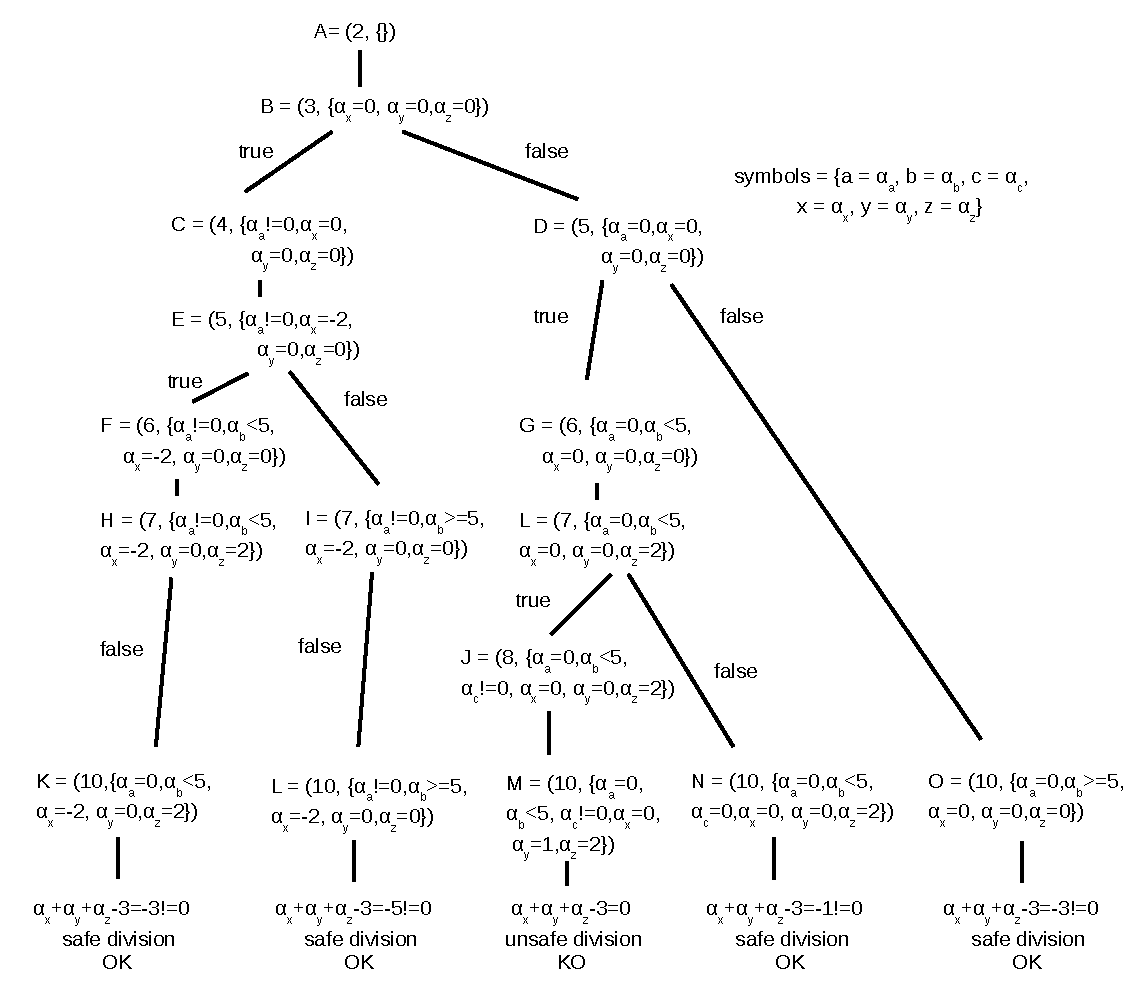
\includegraphics[width=1.0\columnwidth]{images/example} 
%  \caption{Symbolic execution tree of the function {\tt foobar}. Each execution state is labeled with an alphabet letter. Side effects on execution states are highlighted in gray. Leaves are evaluated against division by zero error. For the sake of presentation the conjunction of constraints is shown as a list of constraints. }
%  \label{fig:example-symbolic-execution}
%\end{figure}

\begin{figure}[t]
  \centering
  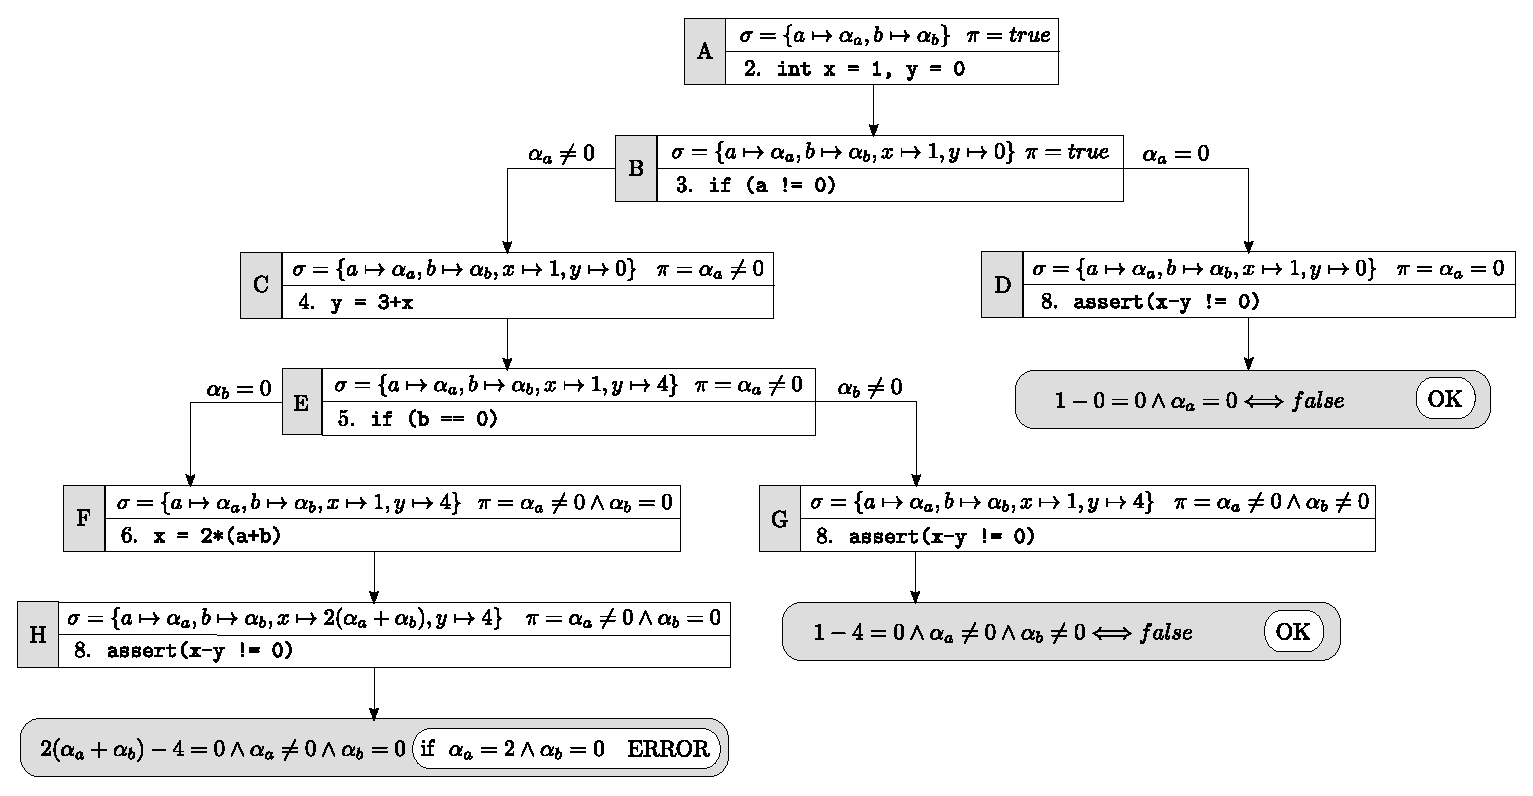
\includegraphics[width=1.0\columnwidth]{images/execution-tree.eps} 
  \caption{Symbolic execution tree of function {\tt foobar} given in Figure~\ref{fig:example-1}. Each execution state, labeled with an upper case letter, shows the statement to be executed, the symbolic store $\sigma$, and the path constraints $\pi$. Leaves are evaluated against the condition in the {\tt assert} statement. }
%For the sake of presentation the conjunction of constraints is shown as a list of constraints. }
  \label{fig:example-symbolic-execution}
  %\vspace{-2mm}
\end{figure}

\noindent A symbolic execution of function {\tt foobar}, which can be effectively represented as a tree, is shown in Figure~\ref{fig:example-symbolic-execution}. Initially (execution state $A$) the path constraints are {\tt true} and input arguments {\tt a} and {\tt b} are associated with symbolic values. 
After initializing local variables {\tt x} and {\tt y} at line 2, the symbolic store is updated by associating {\tt x} and {\tt y} with concrete values 1 and 0, respectively (execution state $B$). Line 3 contains a conditional branch and the execution is forked: depending on the branch taken, a different statement is evaluated next and different assumptions are made on symbol $\alpha_a$ (execution states $C$ and $D$, respectively). In the branch where $\alpha_a\neq 0$, variable {\tt y} is assigned with ${\tt x}+3$, obtaining $y\mapsto 4$ in state $E$ because $x\mapsto 1$ in state $C$. In general, arithmetic expression evaluation simply manipulates the symbolic values.
After expanding every execution state until the {\tt assert} at line 8 is reached on all branches, we can check which input values for parameters {\tt a} and {\tt b} can make the {\tt assert} fail. By analyzing execution states $\{D,G,H\}$, we can conclude that only $H$ can make {\tt x-y = 0} true. The path constraints for $H$ at this point implicitly define the set of inputs that are unsafe for {\tt foobar}. 
In particular, any input values such that:
 \[ 2(\alpha_a+\alpha_b)-4 = 0 \wedge \alpha_a \neq 0 \wedge \alpha_b = 0 \]
will make {\tt assert} fail. An instance of unsafe input parameters can be eventually determined by invoking an {\em SMT solver}~\cite{BKM14} to solve the path constraints, which in this example would yield $a = 2$ and $b = 0$. % HandbookOfSAT2009

%Notice\mynote{Say earlier?} that a constraint solver is also needed when evaluating the satisfiability of branch conditions.

% --------------------------------------------------------------------------------------------------------------------
\subsection{Challenges in Symbolic Execution}
\label{example-discussion}

In the example discussed in Section~\ref{symbolic-execution-example} symbolic execution can identify {\em all} the possible unsafe inputs that make the {\tt assert} fail. This is achieved through an exhaustive exploration of the possible execution states. From a theoretical perspective, exhaustive symbolic execution provides a {\em sound} and {\em complete} methodology for any decidable analysis. Soundness prevents false negatives, i.e., all possible unsafe inputs are guaranteed to be found, while completeness prevents false positives, i.e.,  input values deemed as unsafe are actually unsafe. As we will discuss later on, exhaustive symbolic execution is unlikely to scale beyond small applications. Hence, in practice we often settle for less ambitious goals, e.g., by trading soundness for performance.

Challenges that symbolic execution has to face when processing real-world code can be significantly more complex than those illustrated in our warm-up example. Several observations and questions naturally arise:

\mytempedit{
\begin{itemize}[itemsep=1mm]
%%%
\item \noindent {\em Memory}: how does the symbolic engine handle pointers, arrays, or other complex objects? Code manipulating pointers and data structures may give rise not only to symbolic stored data, but also to addresses being described by symbolic expressions.
%Any arbitrarily complex object can be regarded as an array of bytes and each byte associated with a distinct symbol. However, when possible, exploiting structural properties of the data may be more convenient: for instance, relational bounds on the class fields in object-oriented languages could be used for refining the search performed by symbolic execution.
%%%
\item {\em Environment and third-party components}: how does the engine handle interactions across the software stack? Calls to library and system code can cause side-effects, e.g., the creation of a file, that could later affect the execution and must be accounted for. However, evaluating any possible interaction outcome may be unfeasible.
%: it would give rise to a large number of states, while only a fraction of them can \mynote{[D] likely?}actually happen in a non-symbolic scenario.
%%\mytempedit{Also, third-party closed-source components and popular frameworks (e.g., Java Swing and Android) pose further challenges to an executor, for instance because of the control flows occurring within them through callbacks.}\mynote{CD: may be dropped if we run out of space}
% Real-world applications constantly interact with the environment (e.g., the file system or the network) through libraries and system calls. These interactions may cause side-effects (such as the creation of a file) that could later affect the execution and must be therefore taken into account. Evaluating any possible interaction outcome is generally unfeasible: it could generate a large number of execution states, of which only a small number can actually happen in a non-symbolic scenario. %A typical strategy is to consider popular library and system routines and create models that can help the symbolic engine analyze only significant outcomes.
%%%
  \item {\em State space explosion}: how does symbolic execution deal with path explosion?
%\mynote{[D] I felt it was too long and loop-centric} 
Language constructs such as loops might exponentially increase the number of execution states. It is thus unlikely that a symbolic execution engine can exhaustively explore all the possible states within a reasonable amount of time. %In practice, heuristics are used to guide exploration and prioritize certain states first (e.g., to maximize code coverage). In addition, 
%\mytempedit{Efficient mechanisms can be implemented for preventing repeated exploration of the same piece of code
%\mytempedit{for skipping over states subsumed by previously explored paths} 
%and for evaluating multiple states in parallel without running out of resources.}
%%A loop\mynote{IF: rimuoverei la prima frase, perche' va detto?} can be encoded using conditional branches and {\tt goto} statements, which is typical  when compiling high-level languages to an intermediate representation or native code. 
%Choosing the number of loop iterations to analyze is especially critical when this number cannot be determined in advance (e.g., depends on an input parameter). The naive approach of unrolling iterations for every valid bound would result in a prohibitively large number of states. Typical solutions are to compute an underapproximation of the analysis by limiting the number of iterations to some value $k$, thus trading speed for soundness. Other approaches infer loop invariants through static analysis  and use them to merge equivalent states. % \mynote{i.e. or e.g.?}  (e.g., when differences are not observable from outside the loop body). 
  %In practice, several heuristics must be exploited to prioritize evaluation of some states, hoping to still be able to spot interesting things. Moreover, the symbolic execution engine should include efficient mechanism for efficiently evaluating in parallel different execution states without running out of computational resources.
%%%
  \item {\em Constraint solving}: what can a constraint solver do in practice?
  %{\em What is a constraint solver in practice}? \\
SMT solvers can scale to complex combinations of constraints over hundreds of variables. However, constructs such as non-linear arithmetic pose a major obstacle to efficiency.
%Constraint solvers suffer from a number of limitations. They can typically handle complex constraints in a reasonable amount of time only if they are made of linear expressions over their constituents.
%Constraint solvers suffer from a number of limitations. They can typically handle complex constraints in a reasonable amount of time only if they are made of linear expressions over their constituents. %Symbolic execution engines normally implement a number of optimizations to make queries as much {\em solver-friendly} as possible, for instance by splitting queries into independent components to be processed separately or by performing algebraic simplifications.
%%%
\iffullver{  \item {\em Binary code}: what issues can arise when symbolically executing binary code?
  %what are the disadvantages of symbolically executing binary code?
 While the warm-up example of Section~\ref{symbolic-execution-example} is written in C, in several scenarios binary code is the only available representation of a program. However, having the source code of an application can make symbolic execution significantly easier, as it can exploit high-level properties (e.g., object shapes) that can be inferred statically by analyzing the source code.
 }{}
%(e.g., the maximum size of a buffer or the number of iterations for a loop).
%%%   
\end{itemize}
%Depending on the specific application context of symbolic execution
}

\noindent Depending on the specific context in which symbolic execution is used, different choices and assumptions are made to address the questions highlighted above. Although these choices typically affect soundness or completeness, in several scenarios a partial exploration of the space of possible execution states may be sufficient to achieve the goal (e.g., identifying a crashing input for an application) within a limited time budget.

%\mynote{Better example?}

%different choices and assumptions are made to address the above questions. Although soundness and completeness of symbolic execution may be negatively affected by these choices, there are several application scenarios where a partial exploration of the possible execution states is sufficient for reaching the ultimate goal (e.g., identify a single input that crashes an application).

% --------------------------------------------------------------------------------------------------------------------
\subsection{Related Work}
\label{ss:related-surveys}

\mytempedit{
Symbolic execution has been the focus of a vast body of literature. As of August 2017, Google Scholar reports 742 articles that include the exact phrase ``symbolic execution'' in the title. Prior to this survey, other authors have contributed technical overviews of the field, such as \cite{PV-JSTTT09} and \cite{CS-CACM13}. \cite{CHEN20131758} focuses on the more specific setting of automated test generation: it provides a comprehensive view of the literature, covering in depth a variety of techniques and complementing the technical discussions with a number of running examples.
%Besides  complementing the technical discussions with a number of running examples, it covers in depth recent techniques for key aspects such as memory modelling, environment interaction, path explosion, and constraint solving.
}




% --------------------------------------------------------------------------------------------------------------------
\subsection{Organization of the Article}
\label{ss:article-organization}

\iffullver{
The remainder of this article is organized as follows. In Section~\ref{se:executors}, we discuss the overall principles and evaluation strategies of a symbolic execution engine. Section~\ref{memory-model} through Section~\ref{se:symbolic-binary} address the key challenges that we listed in Section~\ref{example-discussion}. Prominent applications based on symbolic execution techniques are discussed in Section~\ref{se:applications}, while concluding remarks are addressed in Section~\ref{se:conclusions}. %We provide a glossary of the main terms used in the article in Section~\ref{se:glossary}.
}
{
\mytempedit{
The remainder of this article is organized as follows. In Section~\ref{se:executors} we discuss the overall principles and evaluation strategies of a symbolic execution engine. Section~\ref{memory-model} through Section~\ref{se:constraint-solving} address the key challenges that we listed in Section~\ref{example-discussion}, while Section~\ref{se:hang} discusses how recent advances in other areas could be applied to enhance symbolic execution techniques. Concluding remarks are addressed in Section~\ref{se:conclusions}. %We provide a glossary of the main terms used in the article in Section~\ref{se:glossary}.
The appendix addresses further challenges that arise when applying symbolic execution to binary code, discusses some prominent applications of symbolic execution, and includes tables listing some prominent tools and techniques.
}
}


%\vspace{2cm}
%\subsection{Removed stuff}
%
%\paragraph{Black-box approach versus white-box approach}
%
%Discussion\mynote{IF: do we really need this?} of black-box approach and white-box approach. Symbolic execution is a white-box technique. Black-box approaches can be very fast but not always effective. White-box approaches can be very effective but are typically slower than black-box techniques. An in-depth discussion of this aspect will be done when we will discuss~\cite{DRILLER-NDSS16}.
%
%\begin{figure}[H]
%  \vspace{-3mm}
%  \centering
%  \begin{subfigure}{.5\textwidth}
%    \centering
%    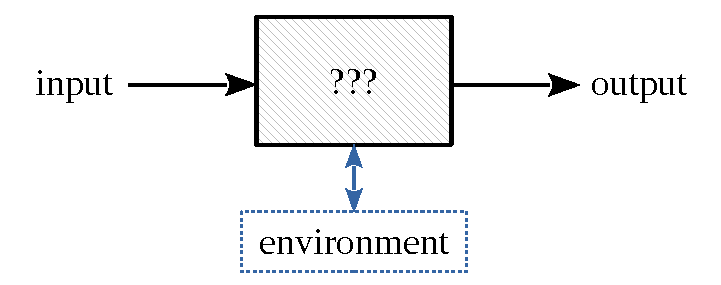
\includegraphics[width=0.9\linewidth]{images/blackbox} 
%    \caption{Black-box approach}
%    %\label{fig:sub1}
%  \end{subfigure}%
%  \begin{subfigure}{.5\textwidth}
%    \centering
%    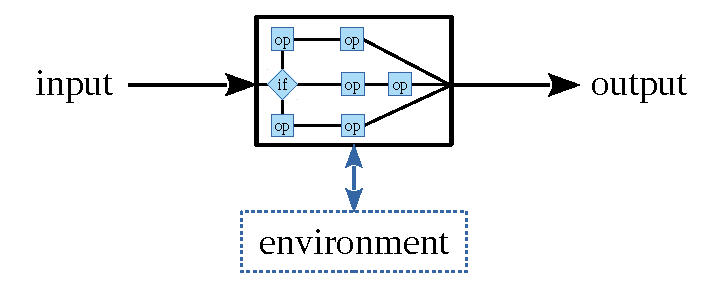
\includegraphics[width=0.9\linewidth]{images/whitebox} 
%    \caption{White-box approach}
%    %\label{fig:sub2}
%  \end{subfigure}
%  %\label{fig:example-symbolic-execution}
%  \vspace{-3mm}
%\end{figure}
%
%\paragraph{Taken from old Overview}
%
%Symbolic execution has been originally introduced in~\cite{K-CACM76} and~\cite{H-TSE77}. A good introduction to symbolic execution is presented in~\cite{KLEE-OSDI08}.\mynote{Extend this paragraph}
%%(while~\cite{EXE-CCS06} is a previous effort of the same authors).
%\cite{SAGE-NDSS08} is one successful story of symbolic execution. \cite{SAB-SP10} presents a neat formalization of symbolic execution and of taint analysis as well.
%
